% Provenance (never printed): see sources/outline_sources.md (Year 2: interstellar
% medium, molecular clouds, gravitational collapse and the Jeans criterion, protostars
% and protostellar discs). Curves from figdata/bachelor-2/jeans.py; exercise and problem
% values in the Book 4 scratch calculator calc/ch01.py.
\chapter{الوسط بين النجمي وتكوّن النجوم}\label{ch:b2:ism-star-formation}

في كوكبة الثور، على بُعد نحو \qty{140}{\parsec} من الشمس، تحجب بقعةٌ داكنة
النجومَ التي خلفها. وحين نرصدها بمقراب راديوي مضبوط على خطوط أحادي أكسيد
الكربون، يتبيّن أنها سحابة من الغاز البارد تفوق كتلتها كتلة الشمس بنحو عشرين
ألف مرة، تتخللها خيوط؛ وفي أكثف عُقَدها تولد نجوم فتيّة، وحول أحدها، إتش إل
الثور، يُظهر قرصٌ من الغبار نمطًا من الحلقات المضيئة والمظلمة قد تكون الكواكب
آخذة في التكوّن فيه. لقد كانت الشمس والأرض وكل ذرّة في صخور هذا الكتاب يومًا
في سحابة كهذه. يتتبّع هذا الفصل مادة نظام كوكبي من الغاز الرقيق بين النجوم
إلى قرص حول نجم وليد: مِمّ يتكوّن \omterm{def:b2:ism-star-formation:ism}{الوسط بين النجمي}، ولماذا تنهار سحابةٌ
تسندها حرارتها الذاتية، وكم يستغرق الانهيار، وكيف يجمع النجم كتلته، ولماذا
تنتهي المادة التي لا تسقط فيه إلى قرص.

\begin{recall}
يسطع النجم على النسق الرئيسي باندماج الهيدروجين إلى هيليوم في
لبّه، ويصمد بضغطه أمام وزنه الذاتي؛ وموقعه في مخطط هرتزشبرونغ--راسل
تحدده كتلته (الفيزياء، السنة الجامعية الثالثة). والجسم الذي يدور في مدار مغلق حول كتلة $M$ يخضع لقانون كبلر
الثالث، $T^2 = 4\pi^2 a^3/(GM)$ (الفيزياء، السنة الجامعية الأولى). والجسم الأسود
الذي درجة حرارته $T$ يُصدر $\sigma T^4$ لكل وحدة مساحة (الفيزياء، السنة الجامعية
الثانية). وفي غاز مثالي من $N$ جسيمًا يساوي متوسط الطاقة الحركية
الانتقالية $\tfrac32 N k_{\mathrm B} T$. والفرسخ الفلكي،
\qty{3.086e16}{m}، هو وحدة المسافة في مجلد السنة الأولى.
\end{recall}

\section{المادة بين النجوم}

ليس الفضاء بين النجوم فارغًا. فبالقرب من الشمس يحوي في المتوسط نحو
ذرّة هيدروجين واحدة في كل سنتيمتر مكعب، أي كثافة كتلية قدرها
\qty{2.7e-24}{g.cm^{-3}}؛ أمّا الهواء الذي نتنفّسه فيحوي نحو $10^{19}$ ضعفًا من
الجزيئات في الحجم نفسه (\cref{exo:b2:ism-star-formation:1}). وحين تتوزّع هذه المادة الرقيقة على المجرّة
تبلغ مع ذلك \qtyrange{10}{15}{\percent} من كتلة
قرص المجرّة.
% ledger: ferriere:mean-density, ferriere:disc-fraction

\begin{definition}[الوسط بين النجمي، الغبار بين النجمي]
\label{def:b2:ism-star-formation:ism}
\emph{الوسط بين النجمي}\index{الوسط بين النجمي} هو الغاز والغبار اللذان
يملآن الفضاء بين نجوم المجرّة. و\emph{الغبار بين
النجمي}\index{الغبار بين النجمي} هو جزؤه الموجود في حبيبات صلبة، يتراوح قطرها بين بضعة
نانومترات ونحو ميكرومتر، مكوّنة من السيليكات ومركّبات الكربون،
وفي المناطق الباردة من الجليد.
\end{definition}

تركيبه هو التركيب المقيس في الشمس وفي النيازك: بالكتلة،
\qty{70.4}{\percent} هيدروجين و\qty{28.1}{\percent} هيليوم
و\qty{1.5}{\percent} عناصر أثقل. ولا يوجد في الغبار سوى \qtyrange{0.5}{1}{\percent} من
الكتلة، ومع ذلك يحتجز الغبار معظم بعض العناصر: فالغاز أفقر من
الشمس في المغنيسيوم والسيليكون والحديد بعوامل تتراوح بين 10 و100، لأن
هذه الذرّات محبوسة في الحبيبات، بينما لا يتجاوز نقص الكربون والنيتروجين والأكسجين
عوامل بين 1.2 و3. والحبيبات هي أولى المواد الصلبة في نظام كوكبي
مقبل؛ ويتتبّعها \cref{ch:b2:planet-formation-meteorites}
لاحقًا.
% ledger: ferriere:composition, ferriere:dust-fraction, ferriere:refractory-depletion

\subsection{خمسة أطوار}

الغاز أبعد ما يكون عن التجانس. فهو يوجد في عدد قليل من الحالات المتمايزة، أو الأطوار،
لكلٍّ منها مداه من درجة الحرارة والكثافة (الجدول أدناه). ونحو نصف
كتلته في سحب لا تشغل إلا \qtyrange{1}{2}{\percent} من الحجم؛
والباقي، الدافئ أو الحار، يملأ الفضاء بينها.
% ledger: ferriere:disc-fraction

\begin{table}[htbp]
\centering
\small
\begin{tabular}{lll}
\hline
الطور & درجة الحرارة (\unit{K}) & الكثافة $n$ (\unit{cm^{-3}}) \\
\hline
جزيئي & \mbox{\textdir TLT 10--20} & \mbox{\textdir TLT $10^2$--$10^6$} \\
ذرّي بارد & \mbox{\textdir TLT 50--100} & \mbox{\textdir TLT 20--50} \\
ذرّي دافئ & \mbox{\textdir TLT 6000--10\,000} & \mbox{\textdir TLT 0.2--0.5} \\
متأيّن دافئ & نحو 8000 & \mbox{\textdir TLT 0.2--0.5} \\
متأيّن حار & نحو $10^6$ & نحو 0.0065 \\
\hline
\end{tabular}
\caption{أطوار الغاز بين النجمي بالقرب من الشمس؛ $n$ هي الكثافة العددية
لنوى الهيدروجين.}
\label{tab:b2:ism-star-formation:phases}
% ledger: ferriere:molecular, ferriere:cold-atomic, ferriere:warm-atomic, ferriere:warm-ionized, ferriere:hot-ionized
\end{table}

يُخفي الجدول انتظامًا. فضغط الغاز المثالي هو
$P = n k_{\mathrm B} T$، ولذلك يقيسه الجداء $nT$. فللغاز الذرّي البارد
يبلغ $nT$ نحو $30\times75 \approx 2000$ (بوحدة \unit{K.cm^{-3}})، وللغاز الذرّي
الدافئ نحو $0.3\times8000 \approx 2400$، وللغاز الحار نحو
$0.0065\times10^6 = 6500$: فالأطوار الثلاثة التي تتقاسم الفضاء بين السحب في الضغط نفسه
تقريبًا، في حدود عامل صغير (الشكل أدناه).
وحيث يتلامس غاز حار وغاز بارد عند ضغط متساوٍ، لا يدفع أحدهما الآخر
بعيدًا؛ والغاز الذي يبرد عند ضغط ثابت تزداد كثافته بالنسبة نفسها
فينتقل من الطور الدافئ إلى الطور البارد. أمّا السحب الجزيئية فتبلغ ضغوطًا أعلى بكثير، تصل إلى آلاف أضعافها في أجزائها الكثيفة: فهي متماسكة بجاذبيتها الذاتية، لا بضغط
محيطها.

\begin{omfigure}
\begin{tikzpicture}
\begin{axis}[omrecord, width=0.86\linewidth, height=6.4cm, xmode=log, ymode=log,
  xmin=1e-3, xmax=1e7, ymin=3, ymax=3e6,
  xlabel={\foreignlanguage{arabic}{كثافة نوى الهيدروجين $n$ \babelsublr{(\unit{cm^{-3}})}}}, ylabel={\foreignlanguage{arabic}{درجة الحرارة $T$ \babelsublr{(\unit{K})}}},
  tick label style={font=\scriptsize}, label style={font=\small}, clip=false,
  legend pos=north east, legend style={font=\scriptsize, draw=black!30}]
\addplot[black!45, densely dashed, domain=1e-3:1e3, samples=2] {3000/x};
\addlegendentry{$nT = \num{3000}$}
\addplot[black!60, densely dotted, thick, domain=0.1:1e5, samples=2] {3e5/x};
\addlegendentry{$nT = 3\times10^5$}
\fill[blue!45, opacity=0.6] (axis cs:1e2,10) rectangle (axis cs:1e6,20);
\fill[teal!50, opacity=0.6] (axis cs:20,50) rectangle (axis cs:50,100);
\fill[orange!55, opacity=0.6] (axis cs:0.2,6000) rectangle (axis cs:0.5,10000);
\fill[red!45, opacity=0.6] (axis cs:0.2,5714) rectangle (axis cs:0.5,11200);
\fill[violet!50, opacity=0.6] (axis cs:0.00464,7.14e5) rectangle (axis cs:0.0091,1.4e6);
\node[font=\scriptsize, anchor=south east] at (axis cs:1e6,20) {السحب الجزيئية};
\node[font=\scriptsize, anchor=south west] at (axis cs:50,100) {ذرّي بارد};
\node[font=\scriptsize, anchor=east, align=right] at (axis cs:0.17,8000) {ذرّي دافئ\\ومتأيّن دافئ};
\node[font=\scriptsize, anchor=west] at (axis cs:0.011,1e6) {متأيّن حار};
\end{axis}
\end{tikzpicture}

\par\smallskip{\small أطوار الغاز بين النجمي بالقرب من الشمس (مدى الجدول
أعلاه؛ أمّا الطوران المتأيّن الدافئ والحار، المعطيان بقيم مفردة، فرُسما مستطيلين
عرضهما عامل 1.4). وعلى طول كل خط رمادي يكون الضغط $nk_{\mathrm B}T$ ثابتًا: فالأطوار
الباردة والدافئة والحارة قريبة من الضغط نفسه، في حدود عامل صغير،
بينما تبلغ السحب الجزيئية، المتماسكة بجاذبيتها الذاتية، ضغوطًا أعلى حتى آلاف المرات.
البيانات: فيريير (2001).}
\end{omfigure}

يكشف الغبار عن نفسه بثلاث طرائق. فهو يُعتم ضوء النجوم التي خلفه،
ويُعتم الضوء الأزرق أكثر من الأحمر، فتبدو النجوم المرئية عبره أشدّ احمرارًا
مما هي عليه. وهو يشعّ في الأشعة تحت الحمراء البعيدة وعند الأطوال الموجية المليمترية،
بدرجة الحرارة البالغة بضع عشرات من الكلفنات التي يدفّئه إليها ضوء النجوم. وهو
يحجب كل ما في داخل السحابة الكثيفة عن المقاريب البصرية، ولهذا
تُرصد عملية تكوّن النجوم بالأطوال الموجية الراديوية وتحت الحمراء. أمّا الغاز
فيُتتبَّع بخطوطه: الهيدروجين الذرّي بخطه الراديوي عند \qty{21}{cm}،
والهيدروجين الجزيئي، الذي لا يكاد يشعّ حين يكون باردًا، بخطوط
الجزيئات المرافقة له، وفي مقدمتها أحادي أكسيد الكربون.

\section{السحب الجزيئية}

الطور الأبرد والأكثف هو حيث تتكوّن النجوم.

\begin{definition}[السحابة الجزيئية، اللبّ الكثيف]
\label{def:b2:ism-star-formation:molecular-cloud}
\emph{السحابة الجزيئية}\index{السحابة الجزيئية} منطقةٌ من
\omterm{def:b2:ism-star-formation:ism}{الوسط بين النجمي} كثيفة ومعتمة بما يكفي لأن يكون معظم هيدروجينها في صورة
جزيئات، \ce{H2}، يحميها الغبار من الأشعة فوق البنفسجية الصادرة عن النجوم
والتي كانت ستفككها؛ ودرجة حرارتها نحو \qty{10}{K} إلى \qty{20}{K}.
و\emph{اللبّ الكثيف}\index{اللبّ الكثيف} تكثّفٌ متراصّ داخل
سحابة جزيئية، لا يتجاوز قطره بضعة أعشار الفرسخ الفلكي، وتتراوح كثافته بين
$10^4$ و$10^5$ جسيم في السنتيمتر المكعب، ويتكوّن منه نجم واحد أو
مجموعة صغيرة من النجوم.
\end{definition}

تنتظم السحب في تراتبية (الجدول أدناه). فالسحابة المظلمة مثل سحابة الثور
تضمّ كُتلًا، وتضمّ الكتلُ لُبوبًا، وكل مستوى أكثف وأصغر وأهدأ
من الذي فوقه: ففي اللبّ يتحرّك الغاز بسرعة لا تزيد على بضعة أعشار
الكيلومتر في الثانية، وهي سرعة الصوت في غاز عند \qty{10}{K}. وتحوي
منطقة الثور المرسومة بأحادي أكسيد الكربون نحو \num{2.4e4} كتلة شمسية
من الغاز؛ ولم يتحوّل منها إلا \qtyrange{0.3}{1.2}{\percent} إلى
النجوم الفتية المرصودة هناك، بمعدل نحو ثمانية نجوم كل مئة ألف
سنة خلال ثلاثة ملايين السنة الأخيرة. فتكوّن النجوم بطيء ومُهدِر.
% ledger: bt07:clouds, bt07:clumps, bt07:cores, goldsmith:taurus-mass, goldsmith:taurus-sfe, goldsmith:taurus-distance

\begin{table}[htbp]
\centering
\small
\begin{tabular}{lccc}
\hline
 & السحب المظلمة & الكتل & اللبوب الكثيفة \\
\hline
الكتلة (كتل شمسية) & \mbox{\textdir TLT $10^3$--$10^4$} & \mbox{\textdir TLT 50--500} & \mbox{\textdir TLT 0.5--5} \\
الحجم (\unit{pc}) & \mbox{\textdir TLT 2--15} & \mbox{\textdir TLT 0.3--3} & \mbox{\textdir TLT 0.03--0.2} \\
متوسط الكثافة (\unit{cm^{-3}}) & \mbox{\textdir TLT 50--500} & \mbox{\textdir TLT $10^3$--$10^4$} & \mbox{\textdir TLT $10^4$--$10^5$} \\
درجة حرارة الغاز (\unit{K}) & نحو 10 & \mbox{\textdir TLT 10--20} & \mbox{\textdir TLT 8--12} \\
أمثلة & الثور، الذبابة & --- & \mbox{\textdir TLT L1544}، \mbox{\textdir TLT B68} \\
\hline
\end{tabular}
\caption{تراتبية سحابة جزيئية مظلمة. تحتسب الكثافات جميع
الجسيمات. البيانات: بيرغن وتافالا (2007).}
\label{tab:b2:ism-star-formation:hierarchy}
% ledger: bt07:clouds, bt07:clumps, bt07:cores
\end{table}

لماذا السحب باردة إلى هذا الحد؟ يفقد الغاز طاقته بإصدار فوتونات
تفلت منه، والجزيئات مُصدِرات كفوءة: فالتصادم يرفع جزيء أحادي أكسيد
الكربون إلى مستوى دوراني أعلى، فيعود الجزيء إلى مستواه بإصدار فوتون
بطول موجي مليمتري، ويغادر الفوتون السحابة
حاملًا معه طاقة التصادم. والغبار، الذي يدفّئه ضوء النجوم الخافت
النافذ إليه، يشعّ في الأشعة تحت الحمراء البعيدة. أمّا التسخين، بالأشعة الكونية
وبضوء النجوم المرشَّح عبر الغبار، فضعيف؛ فيستقر التوازن
قرب \qty{10}{K}. وفي غاز كهذا يكون الضغط الحراري صغيرًا، ويمكن للجاذبية
أن تنتصر.

\begin{omfigure}
\begin{minipage}[c]{0.44\linewidth}
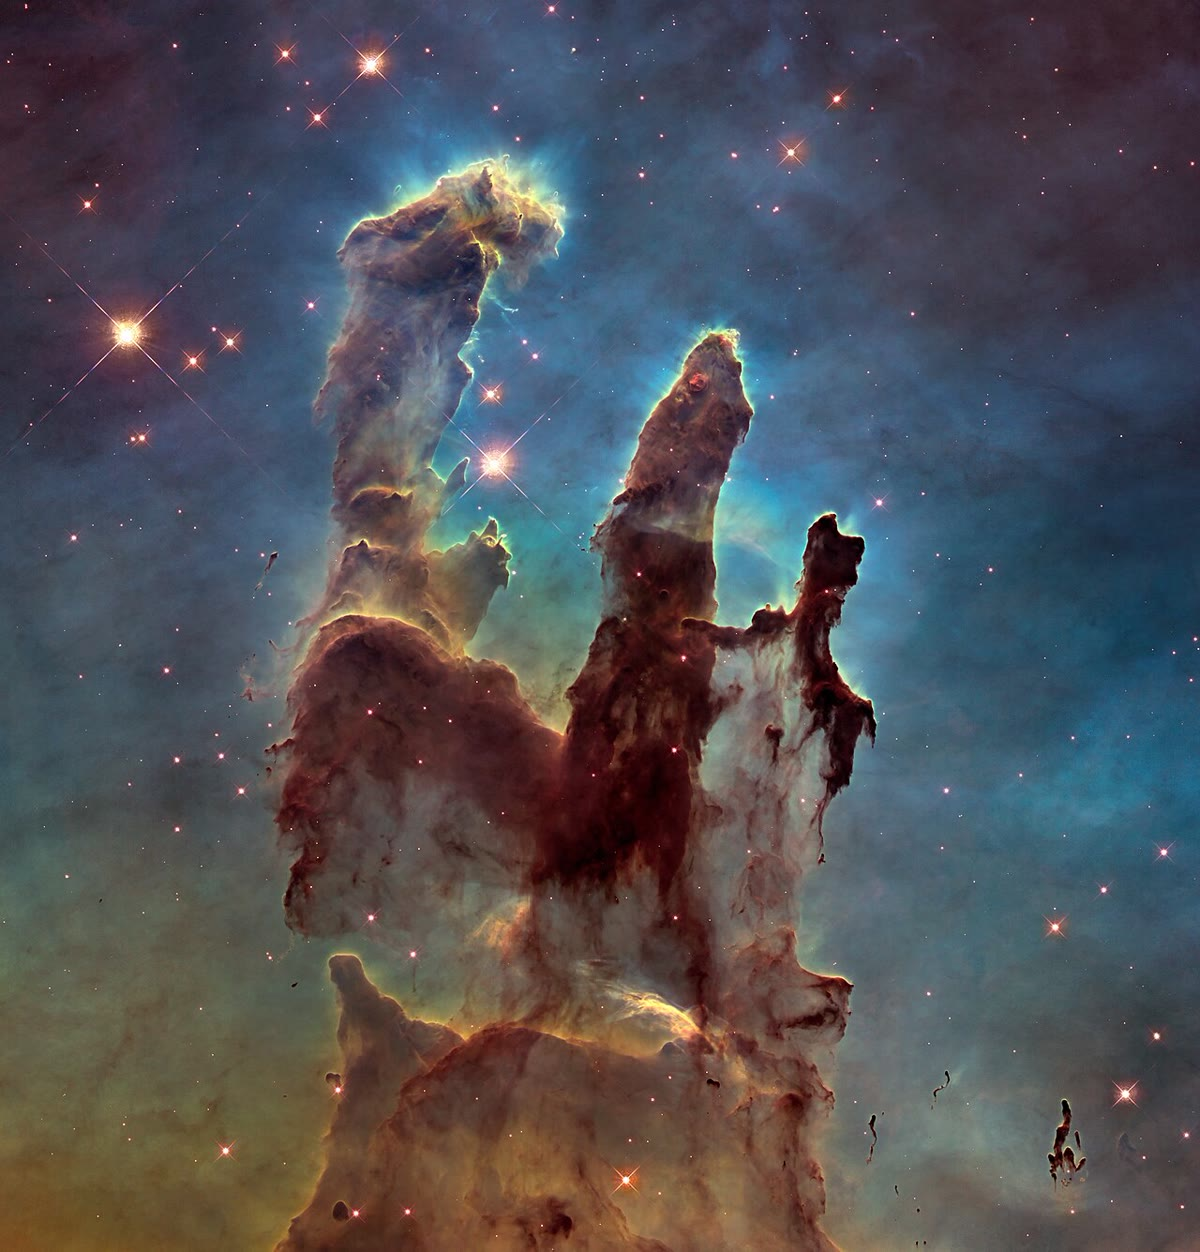
\includegraphics[width=\linewidth]{images/book4/b2-pillars-of-creation.jpg}
\end{minipage}\hfill
\begin{minipage}[c]{0.52\linewidth}
{\small «أعمدة الخلق» في سديم النسر، صوّرها مقراب
هابل الفضائي في الضوء المرئي. الأعمدة غاز جزيئي بارد كثيف
وغبار، طولها سنوات ضوئية، تتآكل وتضاء من الأعلى بالأشعة فوق البنفسجية الصادرة عن
نجوم فتية ضخمة خارج الصورة؛ والغبار يجعلها معتمة. والتكثّفات الصغيرة
عند أطرافها تكوّن نجومًا. \babelsublr{NASA, ESA and the Hubble
Heritage Team (STScI/AURA)}، ملك عام.}
\end{minipage}
\end{omfigure}

\section{الانهيار الثقالي}

السحابة توازنٌ بين طاقتين: الطاقة الحرارية لغازها،
التي تدفع نحو الخارج، وطاقتها الثقالية، التي تشدّ نحو الداخل. والثانية
تنمو مع الكتلة أسرع من الأولى؛ فما فوق كتلةٍ معيّنة تنتصر
الجاذبية.

\begin{proposition}[الطاقة الثقالية لكرة متجانسة]
\label{prop:b2:ism-star-formation:grav-energy}
للكرة المتجانسة الكثافة، التي كتلتها $M$ ونصف قطرها $R$،
طاقة كامنة ثقالية
\[
  U = -\frac{3}{5}\,\frac{G M^2}{R}.
\]
\end{proposition}

\begin{proof}
لنبنِ الكرة قشرةً قشرة. حين يكون نصف قطرها $r$ تكون كتلتها
$m(r) = M r^3/R^3$؛ وجلب قشرة سُمكها $\mathrm dr$ وكتلتها
$\mathrm dm = 3M r^2\,\mathrm dr/R^3$ من اللانهاية إلى سطحها يحرّر
الطاقة $G m(r)\,\mathrm dm/r$، لأن الكرة تجذب ما هو خارجها كما لو كانت
كتلتها مركّزة في مركزها (مبرهنة القشرة، الفيزياء). ومنه
\[
  U = -\int_0^R \frac{G}{r}\,\frac{M r^3}{R^3}\,\frac{3 M r^2}{R^3}\,\mathrm dr
    = -\frac{3 G M^2}{R^6}\int_0^R r^4\,\mathrm dr = -\frac{3}{5}\,\frac{G M^2}{R}.
  \qedhere
\]
\end{proof}

يخضع الجسم المتجاذب ذاتيًا في حالة التوازن لمبرهنة الفيريال: بالمتوسط
على الزمن، ضعف طاقته الحركية مضافًا إليه طاقته الثقالية يساوي صفرًا،
$2K + U = 0$ (الفيزياء، السنة الجامعية الثالثة، حيث تُستنتج من
معادلات الحركة). وللسحابة الساكنة تكون $K$ هي الطاقة الحرارية
لجسيماتها. فإذا كان $2K > |U|$ تمدّد الغاز؛ وإذا كان $2K < |U|$ لم يبقَ للجاذبية
توازنٌ يعارضها فتنكمش السحابة.

\begin{proposition}[معيار جينز]\label{prop:b2:ism-star-formation:jeans}
تنهار سحابة متجانسة متساوية الحرارة، درجة حرارتها $T$ وكثافتها $\rho$، ومكوّنة من
جسيمات متوسط كتلتها $\mu m_u$، تحت جاذبيتها الذاتية إذا تجاوزت كتلتها
\emph{\omterm{def:b2:ism-star-formation:jeans}{كتلة جينز}}
\[
  M_J = \left(\frac{5 k_{\mathrm B} T}{G\mu m_u}\right)^{3/2}
        \left(\frac{3}{4\pi\rho}\right)^{1/2},
\]
أو، على نحو مكافئ، إذا تجاوز نصف قطرها \emph{\omterm{def:b2:ism-star-formation:jeans}{طول جينز}}
\[
  R_J = \left(\frac{15 k_{\mathrm B} T}{4\pi G\mu m_u\,\rho}\right)^{1/2}.
\]
هذا هو \emph{معيار جينز}\index{معيار جينز}.
\end{proposition}

\begin{proof}
تحوي السحابة $N = M/(\mu m_u)$ جسيمًا، طاقتها الحرارية
$K = \tfrac32 N k_{\mathrm B}T = \tfrac32 M k_{\mathrm B}T/(\mu m_u)$. وحسب
\cref{prop:b2:ism-star-formation:grav-energy}، تنهار السحابة إذا كان
$2K < \tfrac35 GM^2/R$، أي
\[
  \frac{3 M k_{\mathrm B} T}{\mu m_u} < \frac{3}{5}\,\frac{G M^2}{R}
  \iff M > \frac{5 k_{\mathrm B} T}{G \mu m_u}\, R .
\]
لنحذف $R$ باستعمال $M = \tfrac43\pi R^3\rho$، أي $R = (3M/4\pi\rho)^{1/3}$:
$M^{2/3} > \frac{5 k_{\mathrm B}T}{G\mu m_u}\,(3/4\pi\rho)^{1/3}$، وبرفع
الطرفين إلى القوة $3/2$ نحصل على $M > M_J$. وإذا حذفنا $M$ بدلًا من ذلك،
فإن $\tfrac43\pi R^3\rho > 5 k_{\mathrm B}T R/(G\mu m_u)$ يعطي $R^2 > 15
k_{\mathrm B}T/(4\pi G\mu m_u\rho)$، أي $R > R_J$.
\end{proof}

\begin{definition}[كتلة جينز، طول جينز]\label{def:b2:ism-star-formation:jeans}
\emph{كتلة جينز}\index{كتلة جينز} $M_J$ و\emph{طول
جينز}\index{طول جينز} $R_J$ لغاز معلوم درجة الحرارة والكثافة
هما الكتلة ونصف القطر اللذان تنهار فوقهما كرةٌ متجانسة من ذلك الغاز
تحت جاذبيتها الذاتية (\cref{prop:b2:ism-star-formation:jeans}).
\end{definition}

تتناسب \omterm{def:b2:ism-star-formation:jeans}{كتلة جينز} مع $T^{3/2}$ ومع $\rho^{-1/2}$: فالغاز البارد الكثيف
ينهار بأكبر سهولة. وفي \omterm{def:b2:ism-star-formation:molecular-cloud}{السحابة الجزيئية} يبلغ متوسط الكتلة لكل جسيم
$\mu = 2.33$ وحدة كتلة ذرّية، أي هيدروجين جزيئي مع ذرّة هيليوم لكل
خمسة جزيئات تقريبًا. وعند \qty{10}{K} و$10^4$ جسيم في السنتيمتر
المكعب، تكون $\rho = \mu m_u n = \qty{3.87e-17}{kg.m^{-3}}$
و$M_J = 5.5$ كتلة شمسية، ضمن \omterm{def:b2:ism-star-formation:jeans}{طول جينز} قدره \qty{0.13}{\parsec}:
وهما كتلة \omterm{def:b2:ism-star-formation:molecular-cloud}{اللبّ الكثيف} وحجمه. وعند متوسط كثافة السحابة المظلمة،
$100$ جسيم في السنتيمتر المكعب، تكون \omterm{def:b2:ism-star-formation:jeans}{كتلة جينز} أكبر بعشر مرات، 55
كتلة شمسية، وتحوي سحابةٌ كتلتها \num{24000} كتلة شمسية مثل سحابة الثور
المئاتِ منها (الشكل أدناه).
% ledger: kauffmann:mu, nist:u, const:kB, const:G, sun:mass, goldsmith:taurus-mass

\begin{omfigure}
\begin{tabular}{@{}c@{\hspace{3mm}}c@{}}
\begin{tikzpicture}
\begin{axis}[omrecord, width=0.455\linewidth, height=6.0cm, xmode=log, ymode=log,
  xmin=10, xmax=1e7, ymin=0.05, ymax=1e4,
  xlabel={$n$ \babelsublr{(\unit{cm^{-3}})}}, ylabel={\foreignlanguage{arabic}{كتلة جينز (كتلة شمسية)}},
  tick label style={font=\scriptsize}, label style={font=\small},
  legend style={font=\scriptsize, at={(0.97,0.97)}, anchor=north east, draw=none, fill=white, fill opacity=0.85}]
\fill[blue!12] (axis cs:1e4,0.5) rectangle (axis cs:1e5,5);
\node[font=\scriptsize, blue!50!black, anchor=north east] at (axis cs:1e5,0.5) {اللبوب الكثيفة};
\addplot[very thick, blue!70!black] table[x=n, y=MJ10] {figdata/out/bachelor-2-jeans-jeans.dat};
\addlegendentry{\mbox{\textdir TLT \qty{10}{K}}}
\addplot[very thick, orange!80!black] table[x=n, y=MJ20] {figdata/out/bachelor-2-jeans-jeans.dat};
\addlegendentry{\mbox{\textdir TLT \qty{20}{K}}}
\addplot[very thick, red!75!black] table[x=n, y=MJ50] {figdata/out/bachelor-2-jeans-jeans.dat};
\addlegendentry{\mbox{\textdir TLT \qty{50}{K}}}
\end{axis}
\end{tikzpicture}
&
\begin{tikzpicture}
\begin{axis}[omrecord, width=0.455\linewidth, height=6.0cm, xmode=log, ymode=log,
  xmin=10, xmax=1e7, ymin=0.01, ymax=20,
  xlabel={$n$ \babelsublr{(\unit{cm^{-3}})}}, ylabel={\foreignlanguage{arabic}{زمن السقوط الحر \babelsublr{(Myr)}}},
  tick label style={font=\scriptsize}, label style={font=\small}]
\addplot[very thick, black!70] table[x=n, y=tff_Myr] {figdata/out/bachelor-2-jeans-tff.dat};
\fill[blue!12] (axis cs:1e4,0.05) rectangle (axis cs:1e5,0.5);
\addplot[very thick, black!70] table[x=n, y=tff_Myr] {figdata/out/bachelor-2-jeans-tff.dat};
\node[font=\scriptsize, blue!50!black, anchor=north] at (axis cs:3.2e4,0.05) {اللبوب};
\end{axis}
\end{tikzpicture}
\\[2pt]
{\small (أ) \omterm{def:b2:ism-star-formation:jeans}{كتلة جينز}} & {\small (ب) \omterm{def:b2:ism-star-formation:free-fall}{زمن السقوط الحر}}
\end{tabular}

\par\smallskip{\small (أ) \omterm{def:b2:ism-star-formation:jeans}{كتلة جينز} بدلالة كثافة الجسيمات لثلاث
درجات حرارة ($\mu = 2.33$). يحدّد المستطيل المظلَّل كتل
اللبوب الكثيفة المرصودة وكثافاتها: فعند \qty{10}{K} تقترب كتلتها من \omterm{def:b2:ism-star-formation:jeans}{كتلة جينز}. (ب) \omterm{def:b2:ism-star-formation:free-fall}{زمن
السقوط الحر} في \cref{prop:b2:ism-star-formation:free-fall}: ثلث مليون
سنة عند $10^4$ جسيم في السنتيمتر المكعب، وأطول بعشر مرات عند $10^2$.}
\end{omfigure}

السحابة التي تبدأ بالانهيار تزداد كثافة، وتتناقص \omterm{def:b2:ism-star-formation:jeans}{كتلة جينز} فيها تناسبًا مع
$\rho^{-1/2}$ ما دامت باردة، وتبقى كذلك ما دامت قادرة على إشعاع
حرارة الانضغاط. فتصبح أجزاء من السحابة غير مستقرة بذاتها
وتنهار كلٌّ على حدة: إنّ السحابة \emph{تتشظّى}. ولهذا تتكوّن النجوم
في مجموعات، ولهذا كتلها صغيرة مقارنةً بالسحب التي تولّدها.
ويتوقف التشظّي حين يصبح الغاز أكثف من أن يسمح لإشعاعه
بالإفلات: فتُحبس حرارة الانضغاط، وترتفع درجة الحرارة، وتكفّ
\omterm{def:b2:ism-star-formation:jeans}{كتلة جينز} عن التناقص.

كم يستغرق الانهيار؟ إذا كان الضغط مهملًا، سقطت كل قشرة من
السحابة سقوطًا حرًّا نحو المركز.

\begin{proposition}[زمن السقوط الحر]\label{prop:b2:ism-star-formation:free-fall}
كرةٌ متجانسة كثافتها $\rho$، ساكنة في البدء وبلا ضغط،
تنهار إلى مركزها في الزمن
\[
  t_{\mathrm{ff}} = \left(\frac{3\pi}{32\,G\rho}\right)^{1/2},
\]
وهو مستقل عن نصف قطرها.
\end{proposition}

\begin{proof}
لنأخذ جسيمًا ساكنًا على البُعد $R$ من المركز، على
سطح الكرة. القشور الداخلية تسقط أسرع منه أو معه، ولا تتخلّف
عنه أبدًا، فتبقى الكتلة $M = \tfrac43\pi R^3\rho$ التي تجذبه ثابتة
طوال المسار. ومساره مدار كبلري منحلّ: قطع ناقص مسطّح حتى صار
قطعة مستقيمة، طرفها البعيد عند $R$ ومركز الجذب عند
طرفها الآخر، فنصف محوره الكبير $a = R/2$. والسقوط من الطرف البعيد
إلى المركز يستغرق نصف دورة؛ وبقانون كبلر الثالث
\[
  t_{\mathrm{ff}} = \frac12\cdot 2\pi\sqrt{\frac{(R/2)^3}{GM}}
  = \pi\sqrt{\frac{R^3}{8\,G\cdot\frac43\pi R^3\rho}}
  = \sqrt{\frac{3\pi}{32\,G\rho}} .
\]
يُختصر $R$: فكل قشرة من الكرة المتجانسة تصل إلى المركز في
اللحظة نفسها.
\end{proof}

\begin{definition}[زمن السقوط الحر]\label{def:b2:ism-star-formation:free-fall}
\emph{زمن السقوط الحر}\index{زمن السقوط الحر} لغاز كثافته $\rho$ هو
$t_{\mathrm{ff}} = (3\pi/32G\rho)^{1/2}$، وهو الزمن الذي تستغرقه كرةٌ متجانسة بتلك
الكثافة لتنهار تحت جاذبيتها الذاتية وحدها.
\end{definition}

يبلغ \omterm{def:b2:ism-star-formation:free-fall}{زمن السقوط الحر} للبّ كثيف من $10^4$ جسيم في السنتيمتر المكعب
\qty{0.34}{Myr}؛ ولسحابة مظلمة كاملة من $10^2$، \qty{3.4}{Myr}. ولو انهارت كل
سحابة جزيئية في المجرّة خلال زمن سقوط حر وتحوّلت إلى
نجوم، لكوّنت المجرّة النجوم أسرع بكثير مما تفعل: ففي سحابة الثور، لا يتجاوز الغاز الذي تحوّل فعلًا
إلى نجوم خلال ثلاثة ملايين السنة الأخيرة نحو واحد في المئة من السحابة.
فالسحب مكبوحة، بالحركات المضطربة وبالحقول المغناطيسية التي يجرّها معه
الجزء المتأيّن من الغاز، ويتبدّد معظم غازها بفعل
رياح النجوم الضخمة الأولى وضوئها قبل أن يتمكّن من الانهيار: ومن هنا
الكفاءة المنخفضة المقيسة في سحابة الثور.
% ledger: bt07:tff

\begin{history}[جيمس جينز]
نشر جيمس جينز (1877--1946) عام 1902 تحليل استقرار
غاز تحت جاذبيته الذاتية الذي تنحدر منه \omterm{def:b2:ism-star-formation:jeans}{كتلة جينز} وطوله. فقد
درس نموّ موجات الكثافة الصغيرة في غاز متجانس لا نهائي
ووجد أن الموجات الأطول من طول حرج لا يعارضها الضغط
بل تنمو: فيتفكك الغاز إلى تكثّفات بذلك الحجم تقريبًا. ولا يختلف طوله
الحرج عن نصف القطر المستنتج أعلاه إلا بعامل عددي؛ أمّا
الفيزياء، أي الجاذبية في مواجهة الضغط الحراري، فهي نفسها.
\end{history}

\section{النجوم الأوّلية}

انهيار اللبّ ليس متجانسًا. فالمركز، الأكثف قليلًا، يسقط
أولًا؛ ويتكوّن هناك جسم صغير كثيف حار ينمو بابتلاع الغاز
الذي لا يكفّ عن الانهمار عليه.

\begin{definition}[النجم الأوّلي]\label{def:b2:ism-star-formation:protostar}
\emph{النجم الأوّلي}\index{النجم الأوّلي} نجمٌ في طور التكوّن لا يزال
يكتسب معظم كتلته بمراكمة غاز لبّه الأم؛ وهو
يسطع بالطاقة التي يحرّرها الغاز الساقط، لا بالاندماج النووي.
\end{definition}

ما سرعة نموّ \omterm{def:b2:ism-star-formation:protostar}{النجم الأوّلي}؟ يحوي اللبّ القريب من الانهيار نحو \omterm{def:b2:ism-star-formation:jeans}{كتلة جينز}
ويسقط في نحو زمن سقوط حر، فتصل الكتلة بمعدل من رتبة
$M_J/t_{\mathrm{ff}}$.

\begin{proposition}[معدل مراكمة النجم الأوّلي]
\label{prop:b2:ism-star-formation:accretion}
لتكن $c_s = (k_{\mathrm B}T/\mu m_u)^{1/2}$ سرعة الصوت متساوية الحرارة
لغاز اللبّ. إن نسبة \omterm{def:b2:ism-star-formation:jeans}{كتلة جينز} إلى \omterm{def:b2:ism-star-formation:free-fall}{زمن السقوط الحر}
لا تتوقف على الكثافة، و
\[
  \frac{M_J}{t_{\mathrm{ff}}} \approx 10\,\frac{c_s^3}{G}:
\]
\omterm{def:b2:ism-star-formation:protostar}{فالنجم الأوّلي} ينمو بمعدل من رتبة $c_s^3/G$، تحدّده درجة حرارة
لبّه وحدها.
\end{proposition}

\begin{proof}
بما أن $k_{\mathrm B}T/(\mu m_u) = c_s^2$، فإن $M_J = 5^{3/2}\,c_s^3\,G^{-3/2}
(3/4\pi\rho)^{1/2}$ و$t_{\mathrm{ff}} = (3\pi/32)^{1/2}(G\rho)^{-1/2}$، ومنه
\[
  \frac{M_J}{t_{\mathrm{ff}}} = 5^{3/2}\left(\frac{3}{4\pi}\right)^{1/2}
  \left(\frac{32}{3\pi}\right)^{1/2}\frac{c_s^3}{G}
  = 11.18\times0.489\times1.84\,\frac{c_s^3}{G} \approx 10\,\frac{c_s^3}{G},
\]
وفيها اختُصرت $\rho$. يتوقف العامل على شكل اللبّ؛
ونماذج اللبوب التي تتناقص كثافتها نحو الخارج، كما هو مرصود، تعطي معدلات
أقرب إلى $c_s^3/G$ نفسها.
\end{proof}

عند \qty{10}{K} تكون $c_s = \qty{0.19}{km.s^{-1}}$ ويبلغ $c_s^3/G$
\num{1.6e-6} كتلة شمسية في السنة: فنجم كالشمس يتجمّع في نحو
\num{600000} سنة، وهو زمن يضاهي \omterm{def:b2:ism-star-formation:free-fall}{زمن السقوط الحر} للبّه.
وفي لبّ أدفأ، عند \qty{20}{K}، يكون المعدل أعلى بعامل $2^{3/2} = 2.8$.

\begin{omfigure}
\begin{tikzpicture}[font=\scriptsize]
% panel 1: core
\begin{scope}
\shade[inner color=gray!70, outer color=gray!10] (0,0) circle (1.0);
\node[align=center] at (0,-1.45) {\foreignlanguage{arabic}{(1) لبّ كثيف}\\$\sim\qty{0.1}{pc}$, \qty{10}{K}};
\end{scope}
% panel 2: collapse with infall arrows
\begin{scope}[xshift=3.0cm]
\shade[inner color=gray!80, outer color=gray!10] (0,0) circle (0.9);
\foreach \a in {0,45,...,315} \draw[-{Stealth[length=1.6mm]}, black!70] (\a:0.85) -- (\a:0.3);
\fill[orange!90!red] (0,0) circle (0.07);
\node[align=center] at (0,-1.45) {\foreignlanguage{arabic}{(2) انهيار}\\$t_{\mathrm{ff}} \sim \qty{0.1}{Myr}$};
\end{scope}
% panel 3: protostar with disc and outflow
\begin{scope}[xshift=6.0cm]
\fill[gray!25] (0,0) ellipse (0.9 and 0.6);
\fill[brown!55] (0,0) ellipse (0.75 and 0.12);
\fill[orange!90!red] (0,0) circle (0.08);
\fill[blue!25] (0,0.1) -- (-0.22,0.95) -- (0.22,0.95) -- cycle;
\fill[blue!25] (0,-0.1) -- (-0.22,-0.95) -- (0.22,-0.95) -- cycle;
\node[align=center] at (0,-1.45) {\foreignlanguage{arabic}{(3) نجم أوّلي وقرص}\\\foreignlanguage{arabic}{وتدفّق ثنائي القطب، $\sim\qty{0.5}{Myr}$}};
\end{scope}
% panel 4: T Tauri with disc
\begin{scope}[xshift=9.0cm]
\fill[brown!55] (0,0) ellipse (0.85 and 0.1);
\fill[yellow!80!orange] (0,0) circle (0.1);
\draw[blue!40, thick] (0,0.15) -- (0,0.6); \draw[blue!40, thick] (0,-0.15) -- (0,-0.6);
\node[align=center] at (0,-1.45) {\foreignlanguage{arabic}{(4) نجم تي الثور}\\\foreignlanguage{arabic}{وقرصه، من 1 إلى \qty{5}{Myr}}};
\end{scope}
% panel 5: planetary system
\begin{scope}[xshift=12.0cm]
\fill[yellow!80!orange] (0,0) circle (0.12);
\foreach \r in {0.3,0.5,0.8} \draw[black!40] (0,0) ellipse ({\r} and {0.4*\r});
\fill (0.3,0) circle (0.03); \fill (-0.5,0.03) circle (0.035); \fill (0.8,0.05) circle (0.06);
\node[align=center] at (0,-1.45) {\foreignlanguage{arabic}{(5) نجم على النسق}\\\foreignlanguage{arabic}{الرئيسي وكواكب}};
\end{scope}
\foreach \x in {1.4,4.4,7.4,10.4} \draw[-{Stealth}, thick, black!60] (\x,0) -- (\x+0.25,0);
\end{tikzpicture}

\par\smallskip{\small من \omterm{def:b2:ism-star-formation:molecular-cloud}{اللبّ الكثيف} إلى النظام الكوكبي (رسم تخطيطي، ليس بمقياس رسم).
(1) لبّ بارد قريب من \omterm{def:b2:ism-star-formation:jeans}{كتلة جينز}. (2) ينهار مركزه أولًا ويتكوّن
نجم أوّلي. (3) ينمو \omterm{def:b2:ism-star-formation:protostar}{النجم الأوّلي} بالمراكمة عبر قرص، بينما يُزيح تدفّقٌ ثنائي القطب
الغازَ على طول محور الدوران. (4) بعد زوال الغلاف، يحيط \omterm{def:b2:ism-star-formation:t-tauri}{بنجم تي الثور}، الذي لا يزال
ينكمش، قرصُه. (5) تبدّد القرص؛ وما بقي من
مواده الصلبة كواكب. الأزمنة مأخوذة من تقديرات السقوط الحر والمراكمة في النص
ومن أعمار الأقراص في القسم الأخير.}
\end{omfigure}

ما دام \omterm{def:b2:ism-star-formation:protostar}{النجم الأوّلي} يراكم المادة فهو يسطع بطاقة الغاز الساقط. فإذا
نفد الغلاف، استمر في السطوع، دون اندماج بعد، بفضل
انكماشه.

\begin{proposition}[الانكماش يمدّ النجم الفتي بالطاقة]
\label{prop:b2:ism-star-formation:contraction}
الكرة الغازية المتجاذبة ذاتيًا في حالة التوازن، إذا انكمشت ببطء، تُشعّ
نصف الطاقة الثقالية التي تحرّرها وتحتفظ بالنصف الآخر حرارةً:
فتزداد سخونة بينما تفقد الطاقة.
\end{proposition}

\begin{proof}
في التوازن تعطي مبرهنة الفيريال $2K + U = 0$، فتكون الطاقة الكلية
$E = K + U = U/2$. فإذا تقلّص نصف القطر تناقصت $U$ بمقدار ما
$\Delta < 0$؛ عندئذ تتغير $E$ بمقدار $\Delta/2$، وهي الطاقة المُشعّة
إلى الخارج، وتتغير $K = -U/2$ بمقدار $-\Delta/2 > 0$: فالطاقة الحرارية، ومعها
درجة الحرارة، ترتفع بالنصف الآخر.
\end{proof}

\begin{definition}[زمن كلفن--هلمهولتز]\label{def:b2:ism-star-formation:kh-time}
\emph{زمن كلفن--هلمهولتز}\index{زمن كلفن--هلمهولتز}
لنجم كتلته $M$ ونصف قطره $R$ وضياؤه $L$ هو
$t_{\mathrm{KH}} = GM^2/(RL)$، وهو رتبة قدر الزمن الذي يستطيع
الانكماش وحده خلاله أن يمدّه بضيائه.
\end{definition}

للشمس الحالية $t_{\mathrm{KH}} = \qty{31}{Myr}$: وهو أقصر بكثير من
عمرها، ولهذا لا بدّ للشمس من أن تحرق الهيدروجين. ولنجم فتيّ كتلته كتلة
شمسية واحدة ونصف قطره ضعف نصف قطر الشمس وضياؤه ضعف ضيائها، يبلغ \qty{8}{Myr}
(\cref{exo:b2:ism-star-formation:6}). وينتهي الانكماش حين يصبح المركز حارًّا بما يكفي لأن يمدّ اندماجُ الهيدروجين
النجمَ بضيائه: فيصل النجم إلى النسق الرئيسي (ما تعرفه من قبل).
% ledger: sun:mass, sun:R, sun:L, const:G

\begin{definition}[نجم تي الثور، التدفّق ثنائي القطب]\label{def:b2:ism-star-formation:t-tauri}
\emph{نجم تي الثور}\index{نجم تي الثور} نجمٌ فتيّ كتلته أقل من نحو
كتلتين شمسيتين، طرح غلافه وأصبح مرئيًا لكنه لم يبلغ
النسق الرئيسي بعد: فهو يسطع بالانكماش، ويتغيّر
لمعانه، ويحيط به عادةً قرص لا يزال يراكم منه
المادة. و\emph{التدفّق ثنائي القطب}\index{التدفّق ثنائي القطب} زوجٌ من النفاثات
أو الرياح الغازية السريعة يقذفها نجم فتيّ في اتجاهين متعاكسين على طول
محور دوران قرصه.
\end{definition}

تحمل التدفّقات بعيدًا جزءًا من الزخم الزاوي للغاز الذي يغذّي به القرصُ
النجمَ، وتُزيح الغلاف على طول المحور؛ ونجم
إتش إل الثور، في نهاية مرحلته النجمية الأوّلية، يدفع تدفّقًا شديد
التسدّد.
% ledger: alma:hltau

\section{الأقراص}

يدور \omterm{def:b2:ism-star-formation:molecular-cloud}{اللبّ الكثيف} ببطء: فعبر اللبّ تتغير سرعة الغاز ببضعة
أعشار الكيلومتر في الثانية لكل فرسخ فلكي. وحين ينهار اللبّ يُحفظ
زخمه الزاوي، فيصير الدوران البطيء سريعًا.

\begin{proposition}[نصف القطر الطارد المركزي]\label{prop:b2:ism-star-formation:centrifugal}
الغاز الذي زخمه الزاوي النوعي $j$ (الزخم الزاوي لكل وحدة كتلة)
والساقط نحو كتلة $M$ لا يستطيع بلوغ المركز: فهو يستقر على مدار
دائري نصف قطره
\[
  r_c = \frac{j^2}{G M}.
\]
\end{proposition}

\begin{proof}
بلا احتكاك يُحفظ الزخم الزاوي للغاز الساقط، فتكون سرعة دورانه
على البُعد $r$ هي $v = j/r$. ويستطيع الغاز الدوران عند $r$ إذا
أمدّته الجاذبية بالتسارع المركزي تمامًا،
$GM/r^2 = v^2/r = j^2/r^3$، أي عند $r = j^2/(GM)$. وأقرب من ذلك يتجاوز
التسارع المركزي المطلوب، $j^2/r^3$، شدّ الجاذبية، فلا
يستطيع الغاز التقدّم أكثر.
\end{proof}

الغاز الساقط على طول محور الدوران قليل الزخم الزاوي فيتجه
مباشرة إلى النجم؛ أمّا الغاز الساقط في المستوي الاستوائي فيحتفظ
بدورانه. والغاز الساقط من جهتين متقابلتين على مسارات مختلفة يتصادم
فوق المستوي الاستوائي وتحته، فيفقد حركته الرأسية، ويتجمّع
في قرص دوّار رقيق نصف قطره نحو $r_c$. وللبّ قطره
\qty{0.1}{pc} يدور دورة واحدة في نحو عشرين مليون سنة، يبلغ $r_c$ بضع
مئات من الوحدات الفلكية (\cref{exo:b2:ism-star-formation:11}): وهو حجم الأقراص المرصودة.

\begin{definition}[القرص الكوكبي الأوّلي]\label{def:b2:ism-star-formation:disc}
\emph{القرص الكوكبي الأوّلي}\index{القرص الكوكبي الأوّلي} (أو
\emph{القرص النجمي الأوّلي}\index{القرص النجمي الأوّلي}) هو القرص المسطّح من
الغاز والغبار الذي يدور دورانًا كبلريًا تقريبًا حول نجم فتيّ، والمكوّن من
مادة لبّه الأم التي احتفظت بزخم زاوي أكبر من أن تسقط على
النجم؛ وفيه تتكوّن الكواكب.
\end{definition}

\begin{omfigure}
\begin{minipage}[c]{0.44\linewidth}
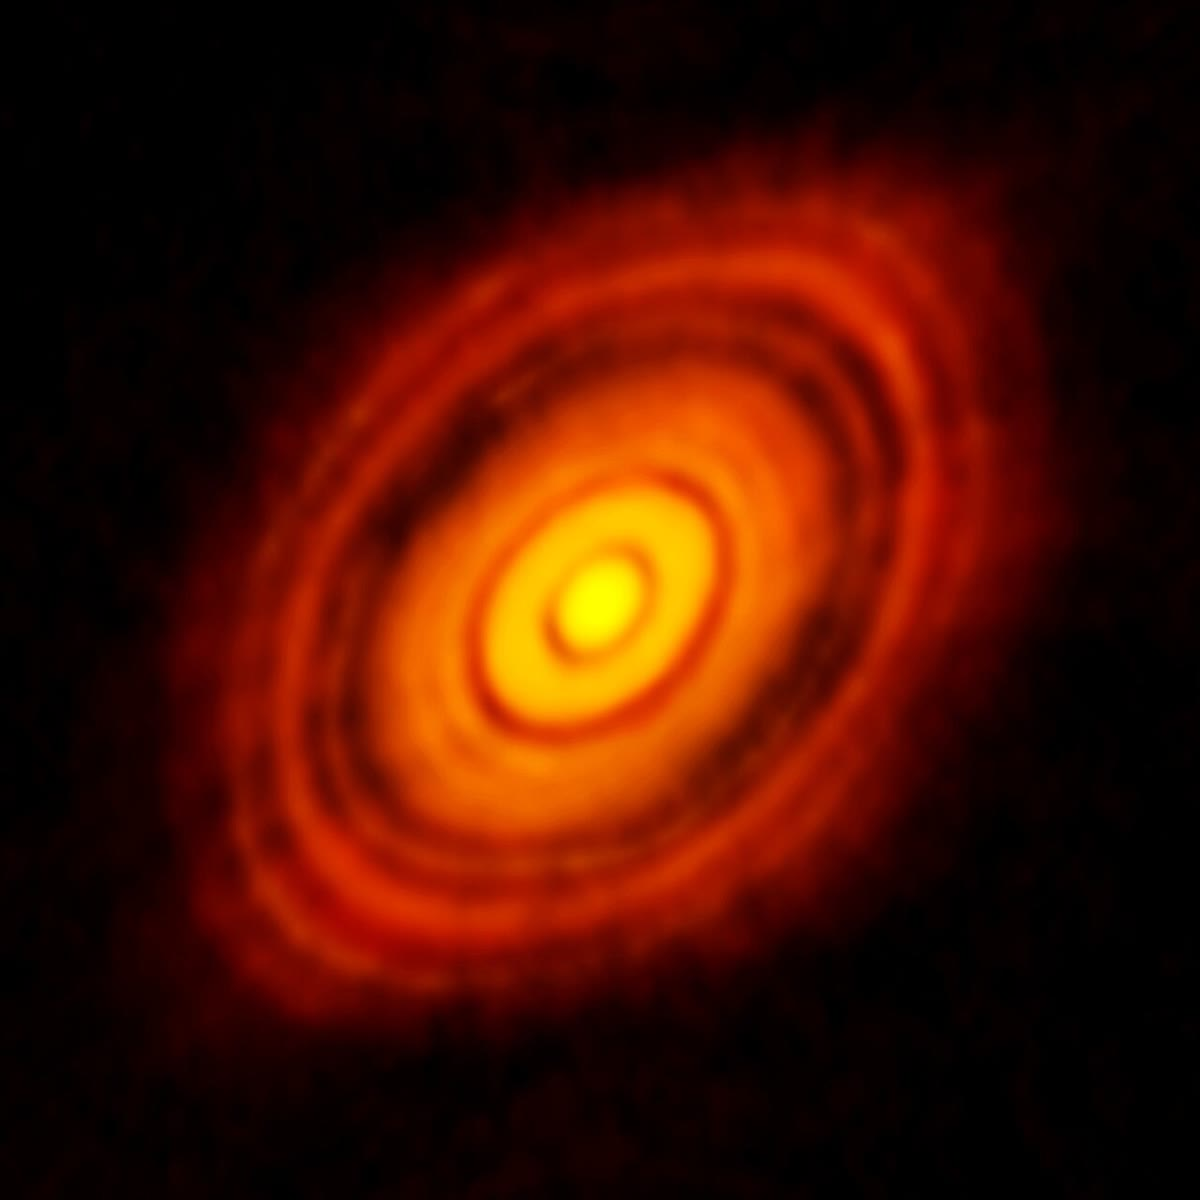
\includegraphics[width=\linewidth]{images/book4/b2-hl-tau-alma.jpg}
\end{minipage}\hfill
\begin{minipage}[c]{0.52\linewidth}
{\small قرص النجم الفتيّ إتش إل الثور، على بُعد \qty{140}{pc} في كوكبة الثور، مصوَّرًا
بمقياس التداخل ALMA عند طول موجي يقارب المليمتر الواحد، حيث يشعّ
الغبار البارد. يُظهر القرص، الذي يبلغ نصف قطره نحو \qty{120}{au} ويُرى مائلًا بزاوية
\ang{47}، حلقات مضيئة ومظلمة عرضها بضع وحدات فلكية؛ ولا يتجاوز عمر
النظام مليون سنة أو مليونين، وتُقرأ الحلقات على أنها
أولى علامات كواكب تشقّ مساراتها. \babelsublr{ALMA (ESO/NAOJ/NRAO)}، \babelsublr{CC BY 4.0}.}
\end{minipage}
% ledger: alma:hltau
\end{omfigure}

يسخّن النجمُ القرصَ. فالحبيبة على البُعد $r$ تمتص ضوء النجم
على مقطعها العرضي وتُشعّ من سطحها كله.

\begin{proposition}[درجة حرارة حبيبة في ضوء النجم]
\label{prop:b2:ism-star-formation:grain}
الحبيبة الصغيرة التي تسلك سلوك الجسم الأسود، على البُعد $r$ من نجم
ضياؤه $L$ والمضاءة من جهة واحدة فقط، تستقر عند درجة الحرارة
\[
  T = \left(\frac{L}{16\pi\sigma r^2}\right)^{1/4},
\]
التي تتناقص تناسبًا مع $r^{-1/2}$.
\end{proposition}

\begin{proof}
الحبيبة الكروية التي نصف قطرها $a$ تعترض القدرة $\pi a^2\,L/(4\pi r^2)$
وتُشعّ، عند درجة الحرارة $T$، القدرة $4\pi a^2\sigma T^4$ من سطحها.
وعند التوازن تتساويان: $T^4 = L/(16\pi\sigma r^2)$؛ وتُختصر $a$.
\end{proof}

على بُعد \qty{1}{au} من نجم كالشمس تكون الحبيبة عند \qty{278}{K}؛ وعلى
\qty{5.2}{au}، حيث يدور المشتري، عند \qty{122}{K}. ويتكاثف جليد الماء حيث
تكون الحبيبات أبرد من نحو \qty{180}{K} (درجات حرارة التكاثف هي
تلك الواردة في \cref{ch:b2:planet-formation-meteorites})، أي فيما وراء نحو
\qty{2.4}{au}: وهي أول علامة على الحدّ، أي خط الثلج، الذي يفصل
الكواكب الصخرية عن الجليدية. والقرص الحقيقي معتم، ومستواه الأوسط محميّ من ضوء النجم المباشر؛ لكن
القضية تعطي رتبة القدر الصحيحة والميل الصحيح
للطبقات السطحية التي يراها النجم.
% ledger: lodders:tc-table

الأقراص لا تدوم. فالفائض تحت الأحمر، أي توهّج الغبار الدافئ فوق ما يُصدره النجم
وحده، يكشف إن كان للنجم قرص بعد. وعدّ النجوم
التي لها هذا الفائض في عناقيد مختلفة الأعمار يعطي نسبة النجوم
التي تحتفظ بقرصها بدلالة الزمن (الشكل أدناه): فلمعظم النجوم قرص
عند الولادة، وقد فقده نصفها في نحو ثلاثة ملايين سنة، ولا يكاد أيٌّ منها
يحتفظ به بعد ستة ملايين. والعمالقة الغازية، التي يجب أن تجمع غازها من القرص،
لا بدّ أن تتكوّن خلال هذه الملايين القليلة من السنين.
% ledger: haisch:disc-fractions, haisch:disc-lifetime

\begin{omfigure}
\begin{tikzpicture}
\begin{axis}[omrecord, width=0.8\linewidth, height=5.6cm, xmin=0, xmax=8.5, ymin=0, ymax=1.05,
  xlabel={\foreignlanguage{arabic}{عمر العنقود \babelsublr{(Myr)}}}, ylabel={\foreignlanguage{arabic}{نسبة النجوم ذات القرص}},
  tick label style={font=\scriptsize}, label style={font=\small}, clip=false]
\addplot[thick, black!55, densely dashed] table[x=age, y=frac] {figdata/out/bachelor-2-jeans-discfit.dat};
\addplot[only marks, mark=*, mark size=1.8pt, blue!70!black,
  error bars/.cd, y dir=both, y explicit]
  table[x=age, y=frac, y error=err, restrict x to domain=0:10] {figdata/out/bachelor-2-jeans-discs.dat};
\node[font=\scriptsize, anchor=north west] at (axis cs:0.05,0.74) {NGC 2024};
\node[font=\scriptsize, anchor=south west] at (axis cs:1.55,0.86) {شبه المنحرف};
\node[font=\scriptsize, anchor=south west] at (axis cs:2.35,0.71) {IC 348};
\node[font=\scriptsize, anchor=south west] at (axis cs:3.3,0.56) {NGC 2264};
\node[font=\scriptsize, anchor=south west] at (axis cs:5.1,0.15) {NGC 2362};
\node[font=\scriptsize, anchor=north east] at (axis cs:8.4,0.98) {\mbox{\textdir TLT (NGC 1960, \qty{30}{Myr}: $0.03$)}};
\end{axis}
\end{tikzpicture}

\par\smallskip{\small نسبة نجوم العناقيد الفتية التي تُظهر الفائض تحت الأحمر
الدالّ على القرص، بدلالة عمر العنقود (مع خطئه)، عن هايش ولادا
ولادا (2001). الخط المتقطّع هو مستقيم المربعات الصغرى المارّ بالعناقيد الخمسة
الأحدث: يبلغ $0.5$ عند \qty{3.0}{Myr} والصفر عند \qty{6.1}{Myr}
(\cref{exo:b2:ism-star-formation:12}).}
\end{omfigure}

\begin{inthelab}[الرؤية عبر الغبار بالموجات الراديوية]
\begin{minipage}[t]{0.55\linewidth}\vspace{0pt}
الغاز والغبار الباردان غير مرئيين للمقاريب البصرية، لكنهما يشعّان عند الأطوال
الموجية المليمترية، حيث لا يكون الغلاف الجوي شفافًا إلا فوق المواقع المرتفعة الجافة.
والطبق الراديوي الذي في حجم منزل لا يميّز إلا القليل عند هذه الأطوال الموجية، ولذلك
يجمع الفلكيون أطباقًا كثيرة: ففي مقياس التداخل يقيس كل زوج من الهوائيات، يفصل بينهما
خط قاعدي، مركّبةً واحدة من نمط سطوع السماء، ثم
يجمّع حاسوب الصورة من مئات الأزواج التي تشكّلها نحو ثلاثين هوائيًا. ودقة التمييز هي دقة
مقراب واحد بعرض أطول خط قاعدي: فبهوائيات موزّعة على
\qty{15}{km} صُوّر قرص إتش إل الثور بتفاصيل تبلغ بضع وحدات فلكية على
\qty{140}{pc}. وينقل المشغّلون الهوائيات على ناقلات بين التشكيلات،
ويجمع جهاز الترابط إشاراتها آنيًا.
\end{minipage}\hfill
\begin{minipage}[t]{0.42\linewidth}\vspace{0pt}
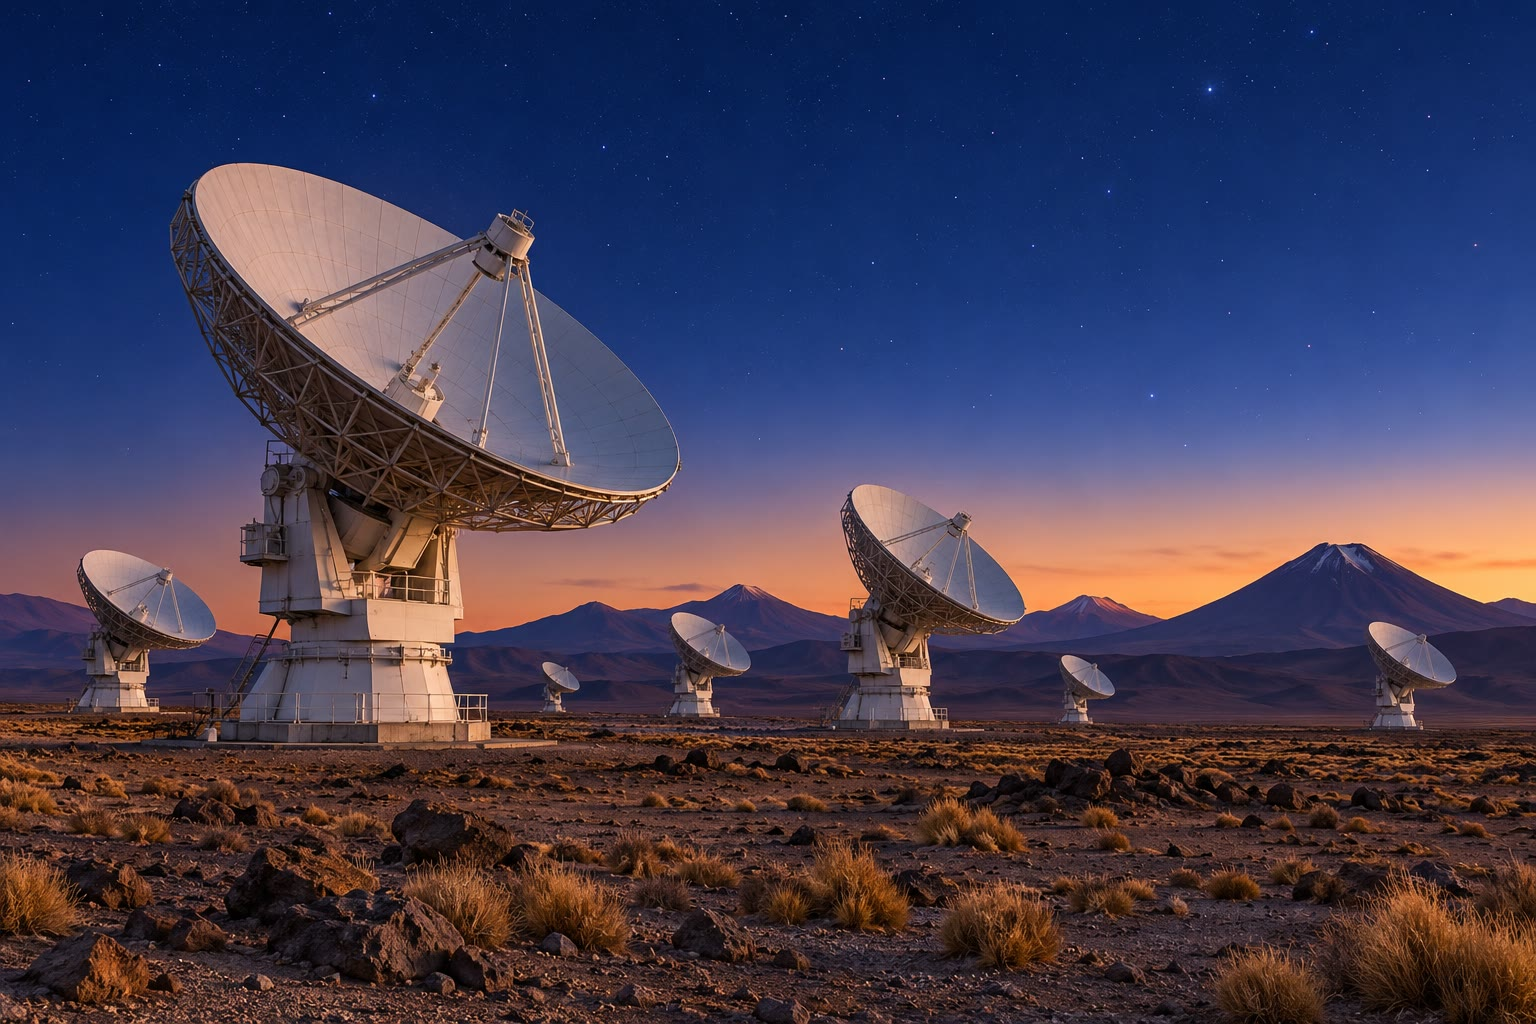
\includegraphics[width=\linewidth]{images/book4/ai/b2-radio-array.jpg}

{\scriptsize صفّ من الهوائيات الراديوية على هضبة صحراوية مرتفعة عند الغسق
(رسم توضيحي مولَّد بالذكاء الاصطناعي).}
\end{minipage}
% ledger: alma:hltau, alma:baselines
\end{inthelab}

\section{التمارين}

\begin{exercise}[$\star$]\label{exo:b2:ism-star-formation:1}
يبلغ متوسط الكثافة بين النجمية قرب الشمس \qty{2.7e-24}{g.cm^{-3}}. باعتبار
كتلة ذرّة الهيدروجين \qty{1.67e-24}{g}، احسب عدد ذرّات الهيدروجين
في السنتيمتر المكعب. وقارنه بعدد الجزيئات في السنتيمتر
المكعب من الهواء عند \qty{101325}{Pa} و\qty{288}{K} ($n = P/k_{\mathrm B}T$).
% ledger: ferriere:mean-density, const:kB
\end{exercise}

\begin{exercise}[$\star$]\label{exo:b2:ism-star-formation:2}
باستعمال القيمة $M_J = 5.46$ كتلة شمسية عند \qty{10}{K} و$10^4$ جسيم
في السنتيمتر المكعب، وقانون تغيّر $M_J$ مع الكثافة، احسب \omterm{def:b2:ism-star-formation:jeans}{كتلة جينز}
عند \qty{10}{K} و$10^2$ جسيم في السنتيمتر المكعب. كم \omterm{def:b2:ism-star-formation:jeans}{كتلة جينز}
تحوي سحابة الثور، البالغة \num{24000} كتلة شمسية؟
% ledger: goldsmith:taurus-mass
\end{exercise}

\begin{exercise}[$\star$]\label{exo:b2:ism-star-formation:3}
احسب سرعة الصوت متساوية الحرارة $c_s = (k_{\mathrm B}T/\mu m_u)^{1/2}$ في
الغاز الجزيئي ($\mu = 2.33$، $m_u = \qty{1.661e-27}{kg}$) عند \qty{10}{K} وعند
\qty{100}{K}. كم تستغرق موجة صوتية لعبور لبّ نصف قطره
\qty{0.1}{pc} عند \qty{10}{K}، بملايين السنين؟
% ledger: kauffmann:mu, nist:u, iau:parsec
\end{exercise}

\begin{exercise}[$\star$]\label{exo:b2:ism-star-formation:4}
احسب \omterm{def:b2:ism-star-formation:free-fall}{زمن السقوط الحر} للبّ كثيف من $10^5$ جسيم في السنتيمتر
المكعب ولسحابة مظلمة من $10^2$ ($\mu = 2.33$). أيّهما ينهار
أسرع، وبأيّ عامل؟
\end{exercise}

\begin{exercise}[$\star\star$]\label{exo:b2:ism-star-formation:5}
بيّن أنه يمكن كتابة $M_J$ على الصورة $M_J = 5^{3/2}\,(3/4\pi)^{1/2}\,c_s^3\,G^{-3/2}\rho^{-1/2}$.
عند درجة حرارة ثابتة، بأيّ عامل يجب أن ترتفع كثافة اللبّ لتنخفض
\omterm{def:b2:ism-star-formation:jeans}{كتلة جينز} إلى النصف؟ وعند كثافة ثابتة، بأيّ عامل تتغير \omterm{def:b2:ism-star-formation:jeans}{كتلة جينز} إذا
سخن اللبّ من \qty{10}{K} إلى \qty{20}{K}؟
\end{exercise}

\begin{exercise}[$\star\star$]\label{exo:b2:ism-star-formation:6}
نجم فتيّ له كتلة الشمس، وضعف نصف قطرها وضعف ضيائها
($M_\odot = \qty{1.989e30}{kg}$، $R_\odot = \qty{6.96e8}{m}$،
$L_\odot = \qty{3.83e26}{W}$). احسب \omterm{def:b2:ism-star-formation:kh-time}{زمن كلفن--هلمهولتز} له بملايين
السنين، وقارنه بأعمار الأقراص.
% ledger: sun:mass, sun:R, sun:L
\end{exercise}

\begin{exercise}[$\star\star$]\label{exo:b2:ism-star-formation:7}
احسب معدل المراكمة $c_s^3/G$ لنجم أوّلي في لبّ عند \qty{10}{K}، بالكتل
الشمسية في السنة، والزمن الذي يستغرقه لجمع كتلة شمسية واحدة. والأسئلة
نفسها للبّ عند \qty{20}{K}.
\end{exercise}

\begin{exercise}[$\star\star$]\label{exo:b2:ism-star-formation:8}
باستعمال \cref{prop:b2:ism-star-formation:grain} و$L_\odot = \qty{3.83e26}{W}$،
احسب البُعد عن الشمس، بالوحدات الفلكية، الذي تبلغ عنده الحبيبة
\qty{1300}{K}، قرب درجة الحرارة التي تتكاثف عندها السيليكات الشائعة
(\cref{ch:b2:planet-formation-meteorites})، واحسب
درجة حرارة حبيبة على بُعد المشتري، \qty{5.2}{au}.
% ledger: sun:L, const:sigma, const:au
\end{exercise}

\begin{exercise}[$\star\star$]\label{exo:b2:ism-star-formation:9}
يدور غاز قرص إتش إل الثور حول نجم كتلته نحو \num{1.3} كتلة
شمسية. احسب السرعة الكبلرية والدور المداري عند \qty{100}{au}.
إذا كان عمر النظام مليون سنة، فكم دورة أتمّ الغاز عند
\qty{100}{au} منذ تكوّن النجم؟
% ledger: alma:hltau
\end{exercise}

\begin{exercise}[$\star\star\star$]\label{exo:b2:ism-star-formation:10}
أوجد الطاقة الثقالية لكرة نصف قطرها $R$ تتناقص فيها الكثافة
وفق $\rho(r) = \rho_0 R/r$، وقارنها بطاقة كرة متجانسة لها
الكتلة ونصف القطر نفساهما. هل يجعل تركّز الكتلة نحو المركز
إسنادَ السحابة بطاقتها الحرارية أسهل أم أصعب؟
\end{exercise}

\begin{exercise}[$\star\star\star$]\label{exo:b2:ism-star-formation:11}
لبٌّ نصف قطره \qty{0.1}{pc} يدور كجسم صلب بالسرعة الزاوية
$\Omega = \qty{1e-14}{rad.s^{-1}}$. احسب دور دورانه، والزخم الزاوي النوعي
$j = \Omega R^2$ للغاز عند خط استوائه، ونصف القطر الطارد المركزي
لذلك الغاز حول نجم كتلته كتلة شمسية واحدة، بالوحدات الفلكية.
لماذا يستقر الغاز الآتي من داخل اللبّ أقرب إلى النجم؟
\end{exercise}

\begin{exercise}[$\star\star\star$]\label{exo:b2:ism-star-formation:12}
نسب الأقراص في العناقيد الخمسة الأحدث في شكل القسم
الأخير هي $0.85$ و$0.80$ و$0.65$ و$0.52$ و$0.12$ عند 0.3 و1.5 و2.3 و3.2
و\qty{5.0}{Myr}. وفّق باليد مستقيم مربعات صغرى $f = a - bt$
(احسب المتوسطات، ثم $\sum(t - \bar t)(f - \bar f)$
و$\sum(t - \bar t)^2$). عند أيّ عمر يبلغ النصف، ثم الصفر؟ ولماذا يكون
المستقيم نموذجًا رديئًا بعد ذلك العمر؟
% ledger: haisch:disc-fractions
\end{exercise}

\section{مسألة: لبٌّ في سحابة ألدرا}

\begin{problem}[{مسألة نهاية الأسبوع --- كتلة لبّ كثيف واستقراره مقروءان من
خريطة الغبار، وولادة نجمه الأوّلي، وحجم قرصه}]
\label{pb:b2:ism-star-formation:1}
% values: calc/ch01.py
% ledger: kauffmann:mu, nist:u, iau:parsec, const:G, const:kB, sun:mass, sun:R, sun:L, const:au, const:sigma, bt07:cores, alma:hltau
سحابة ألدرا سحابة مظلمة متخيَّلة. تُظهر خريطة مليمترية لغبارها
لبًّا مستديرًا نصف قطره \qty{0.08}{pc}، ومتوسط كثافته العمودية
$N(\ce{H2}) = \num{1.5e22}$ جزيء هيدروجين في السنتيمتر المربع. ويعطي
خطٌّ للأمونيا درجة حرارة الغاز، \qty{10}{K}، وتدرّجًا في السرعة
قدره \qty{0.4}{km.s^{-1}} لكل فرسخ فلكي عبر اللبّ، يُقرأ دورانًا
صلبًا. استعمل $G = \qty{6.674e-11}{m^3.kg^{-1}.s^{-2}}$
و$k_{\mathrm B} = \qty{1.381e-23}{J.K^{-1}}$ و$m_u = \qty{1.661e-27}{kg}$
و\qty{1}{pc} $= \qty{3.086e16}{m}$ و\qty{1}{au} $= \qty{1.496e11}{m}$ وسنة طولها
\qty{3.156e7}{s} و$M_\odot = \qty{1.989e30}{kg}$ و$R_\odot = \qty{6.96e8}{m}$
و$L_\odot = \qty{3.83e26}{W}$ و$\sigma = \qty{5.67e-8}{W.m^{-2}.K^{-4}}$؛ وكتلة
جزيء الهيدروجين الواحد، بما فيها الهيليوم، هي $2.8\,m_u$، ومتوسط الكتلة
لكل جسيم $2.33\,m_u$.

\medskip
\noindent\textbf{الجزء الأول --- الكتلة والكثافة.}
\begin{enumerate}
  \item حوّل نصف قطر اللبّ إلى أمتار.
  \item احسب كتلة العمود لكل متر مربع، $2.8\,m_u N$.
  \item استنتج كتلة اللبّ، بالكيلوغرام وبالكتل الشمسية.
  \item احسب حجمه ومتوسط كثافته.
  \item احسب عدد الجسيمات في السنتيمتر المكعب.
  \item هل هذا لبّ كثيف بمعنى جدول القسم الثاني؟
\end{enumerate}

\noindent\textbf{الجزء الثاني --- الاستقرار.}
\begin{enumerate}[resume]
  \item احسب \omterm{def:b2:ism-star-formation:jeans}{كتلة جينز} لغاز اللبّ، بالكتل الشمسية.
  \item كم \omterm{def:b2:ism-star-formation:jeans}{كتلة جينز} يحوي اللبّ؟ وهل هو مستقر؟
  \item احسب \omterm{def:b2:ism-star-formation:jeans}{طول جينز} وقارنه بنصف قطر اللبّ.
  \item كم كانت ستبلغ \omterm{def:b2:ism-star-formation:jeans}{كتلة جينز} لو كان الغاز عند \qty{20}{K}؟ وهل كان
        اللبّ سينهار عندئذ؟
  \item احسب \omterm{def:b2:ism-star-formation:free-fall}{زمن السقوط الحر} للبّ، بآلاف السنين.
  \item قارنه بالزمن الذي تستغرقه موجة صوتية لعبور اللبّ. أيّ
        العمليتين أسرع، وماذا يعني ذلك؟
\end{enumerate}

\noindent\textbf{الجزء الثالث --- \omterm{def:b2:ism-star-formation:protostar}{النجم الأوّلي}.}
\begin{enumerate}[resume]
  \item احسب سرعة الصوت في اللبّ.
  \item احسب معدل المراكمة $c_s^3/G$، بالكتل الشمسية في السنة.
  \item احسب الزمن اللازم لجمع كتلة شمسية واحدة بهذا المعدل.
  \item إذا انتهى ثلث اللبّ إلى نجوم، فكم نجمًا كتلته كتلة شمسية واحدة
        يمكن أن يكوّن؟
  \item بعد زوال الغلاف تصبح للنجم كتلة شمسية واحدة وثلاثة أنصاف أقطار
        شمسية وأربعة أضعاف ضياء الشمس. احسب \omterm{def:b2:ism-star-formation:kh-time}{زمن كلفن--هلمهولتز} له.
  \item هل هو أطول من زمن المراكمة أم أقصر؟ وأيّ نوع من النجوم يكون
        عندئذ؟
\end{enumerate}

\noindent\textbf{الجزء الرابع --- القرص.}
\begin{enumerate}[resume]
  \item حوّل تدرّج السرعة إلى سرعة زاوية $\Omega$، بوحدة
        \unit{rad.s^{-1}}.
  \item احسب الزخم الزاوي النوعي $j = \Omega R^2$ للغاز عند
        خط استواء اللبّ.
  \item احسب نصف قطره الطارد المركزي حول نجم كتلته كتلة شمسية واحدة، بالوحدات
        الفلكية.
  \item احسب درجة حرارة حبيبة على بُعد \qty{1}{au} وعلى بُعد \qty{30}{au}
        من نجم ضياؤه ضياء شمسي واحد.
  \item أين يقع خط الثلج في هذا القرص، إذا كان جليد الماء يبقى دون
        \qty{180}{K}؟
  \item اذكر الزمن اللازم لتجميع نجم السؤال 15، وهو الرقم الأساسي
        في هذه المسألة، بآلاف السنين، وقارنه \omterm{def:b2:ism-star-formation:free-fall}{بزمن
        السقوط الحر} في السؤال 11.
\end{enumerate}
\end{problem}
